% !TEX program = pdflatex
% Statistical Physics Homework_5
\documentclass[12pt,a4paper]{article}
\usepackage[margin=1in]{geometry} 
\usepackage{amsmath,amsthm,amssymb,amsfonts,enumitem,fancyhdr,color,comment,graphicx,environ}
\pagestyle{fancy}
\setlength{\headheight}{65pt}
\newenvironment{problem}[2][Problem]{\begin{trivlist}
\item[\hskip \labelsep {\bfseries #1}\hskip \labelsep {\bfseries #2.}]}{\end{trivlist}}
\newenvironment{sol}
    {\emph{Solution:}
    }
    {
    \qed
    }
\specialcomment{com}{ \color{blue} \textbf{Comment:} }{\color{black}}
\NewEnviron{probscore}{\marginpar{ \color{blue} \tiny Problem Score: \BODY \color{black} }}
\usepackage[UTF8]{ctex}
\usepackage{bm}
\lhead{Name: 陈稼霖\\ StudentID: 45875852}
\rhead{PHYS1503 \\ Statistical Physics \\ Semester Fall 2019 \\ Assignment 5}
\begin{document}
\begin{problem}{7.4}
试证明,对于遵从玻尔兹曼分布的定域系统,熵函数可以表示为
\[
S=-Nk\sum_sP_s\ln P_s
\]
式中$P_s$是粒子处在量子态$s$的概率,$P_s=\frac{e^{-\alpha-\beta\varepsilon_s}}{N}=\frac{e^{-\beta\varepsilon_s}}{Z_1}$,$\sum_s$对粒子的所有量子态求和。\\
对于满足经典极限条件的非定域系统,熵的表达式有何不同?
\end{problem}
\begin{sol}
满足玻尔兹曼分布的定域系统的熵为
\begin{align}
\nonumber S=&Nk\left(\ln Z_1-\beta\frac{\partial}{\partial\beta}\ln Z_1\right)\\
\nonumber=&Nk(\ln Z_1+\beta\frac{U}{N})\\
=&Nk(\ln Z_1+\beta\bar{\varepsilon})
\end{align}
其中配分函数可表为
\begin{equation}
Z_1=\frac{e^{-\beta\varepsilon_s}}{P_s}
\end{equation}
粒子平均能量可表为
\begin{equation}
\bar{\varepsilon}=\sum_sP_s\varepsilon_s
\end{equation}
将以上两式代入熵表达式可得
\begin{align}
\nonumber S=&Nk\sum_sP_s(\ln\frac{e^{-\beta\varepsilon_s}}{P_s}-\beta\varepsilon_s)\\
\nonumber=&Nk\sum_sP_s(-\beta\varepsilon_s-\ln P_s+\beta\varepsilon_s)\\
=&-Nk\sum_sP_s\ln P_s
\end{align}
对于满足经典极限条件的非定域系统,其熵为
\begin{align}
\nonumber S=&Nk\left(\ln Z_1-\beta\frac{\partial}{\partial\beta}\ln Z_1\right)-k\ln N!\\
\nonumber=&-Nk\sum_sP_s\ln P_s-k\ln N!\\
=&-Nk\sum_sP_s\ln P_s-Nk(\ln N-1)
\end{align}
\end{sol}

\begin{problem}{7.6}
晶体含有$N$个原子。原子在晶体中的正常位置如图7.7中的\LARGE$\circ$\normalsize所示。当原子离开正常位置而占据图中的$\times$位置时,晶体中就出现空位和间隙原子。晶体的这种缺陷称为福仑克尔(Frenkel)缺陷。(a)假设正常位置和间隙位置数都是$N$,试证明由于在晶体中形成$n$个空位和间隙原子而具有的熵等于
\[
S=2k\ln\frac{N!}{n!(N-n)!}
\]
\begin{figure}[h]
\centering
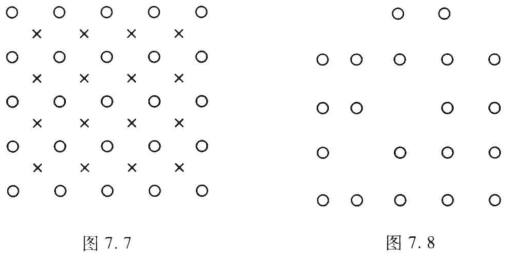
\includegraphics[scale=1]{fig7-7,8.png}
\end{figure}
\\(b)设原子在间隙位置和正常位置的能量差为$u$。试由自由能$F=nu-TS$为极小,证明温度为$T$时,空位和间隙原子数为
\[
n\approx Ne^{-\frac{u}{2kT}},\quad(\text{设}n\ll N)
\]
\end{problem}
\begin{sol}
\begin{itemize}
\item[(a)] 当晶体中形成$n$个空位和间隙原子时,系统可能的微观状态数为
\begin{equation}
\Omega=\left(\begin{array}{c}N\\n\end{array}\right)\left(\begin{array}{c}N\\n\end{array}\right)=\frac{N!}{n!(N-n)!}\frac{N!}{n!(N-n)!}
\end{equation}
故此时系统的熵为
\begin{equation}
S=k\ln\Omega=2k\ln\frac{N!}{n!(N-n)!}
\end{equation}
\item[(b)] 当形成空位和间隙原子时,系统的内能为
\begin{equation}
U=nu+U_0
\end{equation}
其中$U_0$为相同温度下,无缺陷时系统的内能。\\
由于晶体中总粒子数$N\gg1$,利用斯特林公式,系统的自由能为
\begin{align}
\nonumber F=&U-TS\\
\nonumber=&nu+U_0-2kT\ln\frac{N!}{n!(N-n)!}\\
=&nu+U_0-2kT[N\ln N-n\ln n-(N-n)\ln(N-n)]
\end{align}
由自由能极小
\begin{gather}
\frac{\partial F}{\partial n}=u-2kT\ln\frac{N-n}{n}=0\\
\Longrightarrow\ln\frac{N-n}{n}=\frac{u}{2kT}
\end{gather}
由于缺陷数量远小于晶体中总粒子数$n\ll N$,从而上式可近似化为
\begin{equation}
n\approx Ne^{-\frac{u}{2kT}}
\end{equation}
\end{itemize}
\end{sol}

\begin{problem}{7.7}
如果原子脱离晶体内部的正常位置而占据表面上的正常位置,构成新的一层,如图7.8所示,晶体将出现缺陷。晶体的这种缺陷成为肖脱基(Shottky)缺陷。以$N$表示晶体中的原子数,$n$表示晶体中的空位数。如果忽略晶体体积的变化,试由自由能为极小的条件证明,温度为$T$时,
\[
n\approx Ne^{-\frac{W}{kT}},\quad(\text{设}n\ll N)
\]
其中$W$为原子在表面位置与正常位置的能量差。
\end{problem}
\begin{sol}
当出现肖脱基缺陷时,原子脱离晶体内部的正常位置而占据表面的正常位置,系统可能的微观状态数为
\begin{equation}
\Omega=\left(\begin{array}{c}N+n\\n\end{array}\right)=\frac{(N+n)!}{n!N!}
\end{equation}
故此时系统的熵为
\begin{equation}
S=k\ln\Omega=k\ln\frac{(N+n)!}{n!N!}
\end{equation}
系统的内能为
\begin{equation}
U=nW+U_0
\end{equation}
其中$U_0$为相同温度下,无缺陷时系统的内能。\\
由于晶体中总粒子数$N\gg1$,利用斯特林公式,系统的自由能为
\begin{align}
\nonumber F=&U-TS\\
\nonumber=&nW+U_0-kT\ln\frac{(N+n)!}{n!N!}\\
=&nW+U_0-kT[(N+n)\ln(N+n)-n\ln n-N\ln N]
\end{align}
由自由能极小
\begin{gather}
\frac{\partial F}{\partial n}=W-kT\ln\frac{N+n}{n}=0\\
\Longrightarrow\ln\frac{N+n}{n}=\frac{W}{kT}
\end{gather}
由于缺陷数量远小于晶体中总粒子数$n\ll N$,从而上式可近似化为
\begin{equation}
n\approx Ne^{-\frac{W}{kT}}
\end{equation}
\end{sol}

\begin{problem}{7.8}
稀薄气体由某种原子构成。原子两个能级能量之差为
\[
\varepsilon_2-\varepsilon_1=h\omega_0
\]
当原子从高能级$\varepsilon_2$跃迁到低能级$\varepsilon_1$到低能级$\varepsilon_1$时将伴随着光的发射。由于气体中原子的速度分布和多普勒效应,光谱仪观察到的不是单一频率$\omega_0$的谱线,而是频率的一个分布,称为谱线的多普勒增宽。试求温度为$T$时多普勒增宽的表达式。
\end{problem}
\begin{sol}
假设原子质量为$m$,初态处于能级$\varepsilon_2$,速度为$\bm{v}_2$,当向$z$轴方向发射能量为$\hbar\omega$,动量为$\hbar\bm{k}$的光子后,跃迁到能级$\varepsilon_1$,速度变为$\bm{v}_1$。\\
动量守恒和能量守恒要求
\begin{gather}
m\bm{v}_1+\hbar\bm{k}=m\bm{v}_2\\
\varepsilon_1+\frac{1}{2}mv_1^2+\hbar\omega=\varepsilon_2+\frac{1}{2}mv_2^2
\end{gather}
取动量守恒式平方并除以$2m$得
\begin{equation}
\frac{1}{2}mv_1^2+\frac{\hbar^2k^2}{2m}+\hbar\bm{v}_1\cdot\bm{k}=\frac{1}{2}mv_2^2
\end{equation}
将上式代入能量守恒式,并利用$\varepsilon_2-\varepsilon_1=\hbar\omega$得
\begin{gather}
\hbar\omega_0=\hbar\omega-\hbar\bm{v}_1\cdot\bm{k}-\frac{\hbar^2k^2}{2m}\\
\Longrightarrow\omega_0=\omega-\frac{v_{1z}\omega}{c}-\frac{\hbar\omega^2}{2mc^2}
\end{gather}
由于$m\sim10^{-26}$kg,$v_{1z}\sim3\times10^2$m$\cdot$s$^{-1}$,$\omega\sim10^{15}$s$^{-1}$,$\frac{v_{1z}}{c}\sim10^{-6}\gg\frac{\hbar\omega}{2mc^2}\sim10^{-9}$,故上式右边第三项可略去,得
\begin{equation}
\omega=\frac{\omega_0}{1-\frac{v_{1z}}{c}}\approx\omega_0\left(1+\frac{v_{1z}}{c}\right)
\end{equation}
$v_{1z}$在速率范围$v_z$至$v_z+dv_z$内的概率
\begin{equation}
f(v_z)dv_z\propto e^{-\frac{m}{2kT}v_z^2}dv_z
\end{equation}
利用$v_z=c\left(\frac{\omega}{\omega_0}-1\right)$将上面的速率分布转换为频率分布
\begin{equation}
F(\omega)d\omega=\frac{e^{-\frac{m}{2kT}\frac{c^2(\omega-\omega_0)^2}{\omega_0^2}}\frac{c}{\omega_0}d\omega}{\int_0^{+\infty}e^{-\frac{m}{2kT}\frac{c^2(\omega-\omega_0)^2}{\omega_0^2}}\frac{c}{\omega_0}d\omega}=\frac{\omega_0\left(\frac{mc^2}{kT}\right)}{\sqrt{2\pi}}e^{-\frac{m}{2kT}\frac{c^2(\omega-\omega_0)^2}{\omega_0^2}}d\omega
\end{equation}
从而谱线多普勒增宽的表达式为
\begin{equation}
F(\omega)=\frac{\omega_0\left(\frac{mc^2}{kT}\right)}{\sqrt{2\pi}}e^{-\frac{m}{2kT}\frac{c^2(\omega-\omega_0)^2}{\omega_0^2}}
\end{equation}
\end{sol}

\begin{problem}{7.11}
表面活性物质的分子在液面上做二维自由运动,可以看做二维气体。试写出在二维气体中分子的速度分布和速率分布,并求平均速率$\bar{v}$、最概然速率$v_m$和均方均根速率$v_s$。
\end{problem}
\begin{sol}
二维气体中分子的速度分布为
\begin{equation}
\frac{m}{2\pi kT}e^{-\frac{m}{2kT}(v_x^2+v_y^2)}dv_xdv_y
\end{equation}
速率分布为
\begin{equation}
\frac{m}{2\pi kT}e^{-\frac{mv^2}{2kT}}vdv\int_0^{2\pi}d\theta=\frac{m}{kT}e^{-\frac{mv^2}{2kT}}vdv
\end{equation}
平均速率为
\begin{equation}
\bar{v}=\int_0^{+\infty}\frac{m}{kT}e^{-\frac{mv^2}{2kT}}v^2dv=\sqrt{\frac{\pi kT}{2m}}
\end{equation}
最概然速率满足
\begin{gather}
\frac{d}{dv}\left(e^{-\frac{mv^2}{2kT}}v\right)=e^{-\frac{mv^2}{2kT}}\left(-\frac{mv^2}{kT}+1\right)=0\\
\frac{d}{dv}\left[e^{-\frac{mv^2}{2kT}}\left(-\frac{mv^2}{kT}+1\right)\right]=e^{-\frac{mv^2}{2kT}}\left[\left(-\frac{mv}{kT}\right)\left(-\frac{mv^2}{kT}+1\right)-\frac{2mv}{kT}\right]<0
\end{gather}
解得最概然速率为
\begin{equation}
v_m=\sqrt{\frac{kT}{m}}
\end{equation}
速率平方的平均值为
\begin{equation}
\overline{v^2}=\int_0^{+\infty}\frac{m}{kT}e^{-\frac{mv^2}{2kT}}v^3dv=\frac{2kT}{m}
\end{equation}
故方均根速率为
\begin{equation}
v_s=\sqrt{\overline{v^2}}=\sqrt{\frac{2kT}{m}}
\end{equation}
\end{sol}

\begin{problem}{7.12}
试根据麦氏速度分布律导出两分子的相对速度$\bm{v}_r=\bm{v}_2-\bm{v}_1$和相对速率$v_r=|\bm{v}_r|$的概率分布,并求相对速率的平均值$\bar{v}_t$。
\end{problem}
\begin{sol}
根据麦氏速度分布律,分子$1$和分子$2$分别处在速度范围$d\bm{v}_1$和$d\bm{v}_2$内的概率为
\begin{equation}
dP=dP_1\cdot dP_2=\left(\frac{m_1}{2\pi kT}\right)^{3/2}e^{-\frac{m_1v_1^2}{2}}d\bm{v}_1\cdot\left(\frac{m_2}{2\pi kT}\right)^{3/2}e^{-\frac{m_2v_2^2}{2kT}}d\bm{v}_2
\end{equation}
上述两个分子的质心速率和相对速度分别为
\begin{gather}
\bm{v}_c=\frac{m_1\bm{v}_1+m_2\bm{v}_2}{m_1+m_2}\\
\bm{v}_r=\bm{v}_2-\bm{v}_1
\end{gather}
由这两个粒子构成的系统动能既可表为
\begin{equation}
E_k=\frac{1}{2}m_1v_1^2+\frac{1}{2}m_2v_2^2
\end{equation}
又可表为
\begin{equation}
E_k=\frac{1}{2}m_cv_c^2+\frac{1}{2}\mu v_r^2
\end{equation}
其中
\begin{gather}
m_c=m_1+m_2\\
\mu=\frac{m_1m_2}{m_1+m_2}
\end{gather}
因此上面的概率可同理表为
\begin{equation}
dP=\left(\frac{m_c}{2\pi kT}\right)^{3/2}e^{-\frac{m_cv_c^2}{2kT}}d\bm{v}_c\cdot\left(\frac{\mu}{2\pi kT}\right)^{3/2}e^{-\frac{\mu}{2kT}}d\bm{v}_r
\end{equation}
其中相对速度的分布为
\begin{equation}
dP_r=\left(\frac{\mu}{2\pi kT}\right)^{3/2}e^{-\frac{\mu v_r^2}{2kT}}d\bm{v}_r
\end{equation}
相对速率的分布为
\begin{equation}
\left(\frac{\mu}{2\pi kT}\right)^{3/2}e^{-\frac{\mu v_r^2}{2kT}}v_r^2dv_{r}d\theta\int_0^{\pi}\sin\theta d\theta\int_0^{2\pi}d\varphi=4\pi\left(\frac{\mu}{2\pi kT}\right)^{3/2}e^{-\frac{\mu v_r^2}{2kT}}v_r^2dv_{r}
\end{equation}
相对速率的平均值为
\begin{equation}
\bar{v}_r=\int_0^{+\infty}4\pi\left(\frac{\mu}{2\pi kT}\right)^{3/2}e^{-\frac{\mu v_r^2}{2kT}}v_r^3dv_3=\frac{8kT}{\pi\mu}
\end{equation}
\end{sol}

\begin{problem}{7.14}
分子从器壁的小孔射出,求在射出的分子束中,分子的平均速率、方均根速率和平均能量。
\end{problem}
\begin{sol}
设器壁法线方向沿$z$轴,在单位时间内碰到单位面积器壁上,速度范围$dv_x,dv_y,dv_z$内的粒子数为
\begin{equation}
d\Gamma(v_x,v_y,v_z)=n\left(\frac{m}{2\pi kT}\right)^{3/2}e^{-\frac{m}{2kT}(v_x^2+v_y^2+v_z^2)}v_xdv_xdv_ydv_z
\end{equation}
速率范围$dv$内的粒子数为
\begin{align}
\nonumber d\Gamma(v)=&\int_0^{\frac{\pi}{2}}d\theta\int_0^{2\pi}d\phi d\Gamma(v_x,v_y,v_z)v^2\sin\theta dv\\
\nonumber=&\int_0^{\frac{\pi}{2}}d\theta\int_0^{2\pi}d\phi n\left(\frac{m}{2\pi kT}\right)^{3/2}e^{-\frac{m}{2kT}(v_x^2+v_y^2+v_z^2)}v_xv^2\sin\theta dv\\
\nonumber=&\int_0^{\frac{\pi}{2}}d\theta\int_0^{2\pi}d\phi n\left(\frac{m}{2\pi kT}\right)^{3/2}e^{-\frac{m}{2kT}(v_x^2+v_y^2+v_z^2)}v^3\sin\theta\cos\theta dv\\
=&\pi n\left(\frac{m}{2\pi kT}\right)^{3/2}e^{-\frac{m}{2kT}v^2}v^3dv
\end{align}
射出的分子束中,分子的平均速率为
\begin{align}
\nonumber\bar{v}=&\frac{\int_0^{+\infty}vd\Gamma}{\int_0^{+\infty}d\Gamma}\\
\nonumber=&\frac{\int_0^{+\infty}e^{-\frac{m}{2kT}v^2}v^4dv}{\int_0^{+\infty}e^{-\frac{m}{2kT}v^2}v^3dv}\\
=&\sqrt{\frac{9\pi kT}{8m}}
\end{align}
速率平方的平均值为
\begin{align}
\nonumber\overline{v^2}=&\frac{\int_0^{+\infty}v^2d\Gamma}{\int_0^{+\infty}d\Gamma}\\
\nonumber=&\frac{\int_0^{+\infty}e^{-\frac{m}{2kT}v^2}v^5dv}{\int_0^{+\infty}e^{-\frac{m}{2kT}v^2}v^3dv}\\
=&\frac{4kT}{m}
\end{align}
故方均根速率为
\begin{equation}
v_s=\sqrt{\overline{v^2}}=\sqrt{\frac{4kT}{m}}
\end{equation}
平均能量为
\begin{equation}
\bar{\varepsilon}=\frac{1}{2}m\overline{v^2}=2kT
\end{equation}
\end{sol}

\begin{problem}{7.16}
已知粒子遵从经典玻尔兹曼分布,其能量表达式为
\[
\varepsilon=\frac{1}{2m}(p_x^2+p_y^2+p_z^2)+ax^2+bx
\]
其中$a$、$b$是常数,求粒子的平均能量。
\end{problem}
\begin{sol}
粒子能量可表为
\begin{equation}
\varepsilon=\frac{1}{2}(p_x^2+p_y^2+p_z^2)+a(x+\frac{b}{2a})^2-\frac{b^2}{4a}
\end{equation}
根据能量均分定理,粒子的平均能量为
\begin{equation}
\bar{\varepsilon}=2kT-\frac{b^2}{4a}
\end{equation}
\end{sol}

\begin{problem}{7.19}
对于双原子分子,常温下$kT$远大于转动的能级间距。试求双原子分子理想气体的转动熵。
\end{problem}
\begin{sol}
双原子分子理想气体分子的配分函数为
\begin{equation}
Z_1^r=\sum_{l=0}^{\infty}(2l+1)e^{-\frac{l(l+1)}{T}\theta_r}
\end{equation}
当$kT$远大于转动的能级间距,满足经典极限条件,令$x=l(l+1)\frac{\theta_r}{T}$,配分函数可近似为
\begin{align}
\nonumber Z_1^r=&\int_0^{\infty}(2l+1)e^{-x}\frac{dx}{(2l+1)(\theta_r/T)}\\
\nonumber=&\frac{T}{\theta_r}\int_0^{\infty}e^{-x}dx\\
=&\frac{T}{\theta_r}=T\frac{2Ik}{\hbar^2}=\frac{2I}{\beta\hbar^2}
\end{align}
其中转动特征温度$\theta_r=\frac{\hbar^2}{2kI}$。\\
转动熵为
\begin{align}
\nonumber S=&Nk\left(\ln Z_1^r-\beta\frac{\partial}{\partial\beta}\ln Z_1^r\right)\\
\nonumber=&Nk\left[\ln\left(\frac{2I}{\beta\hbar^2}\right)+1\right]\\
=&Nk\left(\ln\frac{T}{\theta_r}+1\right)
\end{align}
\end{sol}

\begin{problem}{7.22}
以$n$表示晶体中原子的密度。设原子的总角动量量子数为$1$,磁矩为$\mu$。在外磁场$B$下,原子磁矩可以有三个不同的取向,即平行、垂直、反平行于外磁场。假设磁矩之间的相互作用可以忽略。试求在温度为$T$时晶体的磁化强度$M$及其在弱场高温极限和强场低温极限下的近似值。
\end{problem}
\begin{sol}
系统中磁矩的配分函数为
\begin{align}
\nonumber Z_1=&\sum_l\overline{\omega_l}e^{-\beta\varepsilon_l}=\sum_l\overline{\omega_l}e^{-\beta\mu_{zl}\mathcal{B}}\\
=&e^{\beta\mu\mathcal{B}}+1+e^{-\beta\mu\mathcal{B}}=1+2\cosh(\beta\mu\mathcal{B})
\end{align}
晶体的磁化强度为
\begin{align}
\nonumber\mathcal{M}=&n\bar{\mu}\\
\nonumber=&\frac{1}{V}\sum_l\mu_{zl}a_l\\
\nonumber=&\frac{1}{V}\sum_l\frac{\partial\varepsilon_l}{-\partial\mathcal{B}}a_l\\
\nonumber=&\frac{1}{V}\frac{N}{\beta}\frac{\partial}{\partial\mathcal{B}}\ln Z_1\\
\nonumber=&\frac{n}{\beta}\frac{\partial}{\partial\mathcal{B}}\ln(1+2\cosh(\beta\mu\mathcal{B}))\\
=&n\mu\frac{2\sinh(\beta\mu\mathcal{B})}{1+2\cosh(\beta\mu\mathcal{B})}
\end{align}
在弱场高温极限下有$\beta\mu\mathcal{B}\ll1\Longrightarrow\sinh(\beta\mu\mathcal{B})\approx\beta\mu\mathcal{B},\cosh(\beta\mu\mathcal{B})\approx1$,故
\begin{equation}
\mathcal{M}=\frac{2}{3}n\beta\mu^2\mathcal{B}
\end{equation}
在强场高温极限下有$\beta\mu\mathcal{B}\gg1\Longrightarrow\sinh(\beta\mu\mathcal{B})\approx\cosh(\beta\mu\mathcal{B})\approx\frac{1}{2}e^{\beta\mu\mathcal{B}}$,故
\begin{equation}
\mathcal{M}=n\mu
\end{equation}
\end{sol}

\begin{problem}{8.2}
试证明,理想玻色和费米系统的熵可分别表示为
\begin{gather*}
S_{B.E.}=-k\sum_s[f_s\ln f_s-(1+f_s)\ln(1+f_s)]\\
S_{F.D.}=-k\sum_s[f_s\ln f_s+(1-f_s)\ln(1-f_s)]
\end{gather*}
其中$f_s$为量子态$s$上的平均粒子数,$\sum_s$对粒子的所有量子态求和,并证明当$f_s\ll1$,有
\[
S_{B.E.}\approx S_{F.D.}\approx S_{M.B.}=-k\sum_s(f_s\ln f_s-f_s)
\]
\end{problem}
\begin{sol}
理想波色系统可能的微观状态数为
\begin{equation}
\Omega_{B.E.}=\prod_l\frac{(\omega_l+a_l-1)!}{a_l!(\omega_l-1)!}
\end{equation}
熵为
\begin{align}
\nonumber S_{B.E.}=&k\ln\Omega_{B.E.}\\
\nonumber=&k\sum_l[(\omega_l+a_l)\ln(\omega_l+a_l)-a_l\ln a_l-\omega_l\ln\omega_l]\\
\nonumber=&-k\sum_l[-(\omega_l+a_l)\ln(\omega_l+a_l)+a_l\ln a_l+(\omega_l+a_l)\ln\omega_l-a_l\ln\omega_l]\\
\nonumber=&-k\sum_l\omega_l[-\frac{\omega_l+a_l}{\omega_l}\ln\frac{\omega+a_l}{\omega_l}+\frac{a_l}{\omega_l}\ln\frac{a_l}{\omega_l}]\\
=&-k\sum_l\omega_l[-(1+\frac{a_l}{\omega_l})\ln(1+\frac{+a_l}{\omega_l})+\frac{a_l}{\omega_l}\ln\frac{a_l}{\omega_l}]
\end{align}
由于平均粒子数
\begin{equation}
f_s=\frac{a_l}{\omega_l}
\end{equation}
故熵可表为
\begin{align}
\nonumber S_{B.E.}=&-k\sum_l\omega_l[f_s\ln f_s-(1+f_s)\ln(1+f_s)]\\
=&-k\sum_s[f_s\ln f_s-(1+f_s)\ln(1+f_s)]
\end{align}
同理,理想费米系统可能的微观状态数为
\begin{equation}
\Omega_{F.D.}=\prod_l\frac{\omega_l!}{a_l!(\omega_l-a_l)!}
\end{equation}
熵为
\begin{align}
\nonumber S_{F.D.}=&-k\ln\Omega_{F.D.}\\
\nonumber=&k\sum_l[\omega_l\ln\omega_l-a_l\ln a_l-(\omega_l-a_l)\ln(\omega_l-a_l)]\\
\nonumber=&-k\sum_l[-(\omega_l-a_l)\ln\omega_l-a_l\ln\omega_l+a_l\ln a_l+(\omega_l-a_l)\ln(\omega_l-a_l)]\\
\nonumber=&-k\sum_l\omega[\frac{\omega_l-a_l}{\omega_l}\ln\frac{\omega_l-a_l}{\omega_l}+\frac{a_l}{\omega_l}\ln\frac{a_l}{\omega_l}]\\
\nonumber=&-k\sum_l\omega[\frac{a_l}{\omega_l}\ln\frac{a_l}{\omega_l}+(1-\frac{a_l}{\omega_l})\ln(1-\frac{a_l}{\omega_l})]\\
\nonumber=&-k\sum_l\omega_l[f_s\ln f_s+(1-f_s)\ln(1-f_s)]\\
=&-k\sum_s[f_s\ln f_s+(1-f_s)\ln(1-f_s)]
\end{align}
当$f_s\ll1$时,有$1\pm f_s\approx1,\ln(1\pm f_s)=\pm f_s$,故
\begin{equation}
S_{B.E.}\approx S_{F.D.}\approx S_{M.B.}=-k\sum_s(f_s\ln f_s-f_s)
\end{equation}
\end{sol}

\begin{problem}{8.4}
试证明,在热力学极限下均匀的二维理想玻色气体不会发生玻色凝聚。
\end{problem}
\begin{sol}
假设能发生玻色凝聚,在其临界温度$T_c$下,玻色系统的化学势满足
\begin{equation}
\frac{1}{V}\sum_l\frac{\omega_l}{e^{\frac{\varepsilon_l-\mu}{kT_c}}-1}=n
\end{equation}
将二维自由粒子的状态密度$D(\varepsilon)d\omega=\frac{2\pi L^2}{h^2}md\varepsilon$代入并将求和换成积分得
\begin{equation}
\int_0^{+\infty}\frac{D(\varepsilon)d\varepsilon}{e^{\frac{\varepsilon}{kT_c}-1}}=\frac{2\pi L^2}{h^2}m\int_0^{+\infty}\frac{d\varepsilon}{e^{\frac{\varepsilon}{kT_c}-1}}=n
\end{equation}
令$x=\frac{\varepsilon}{kT_c}$,上式化为
\begin{equation}
\frac{2\pi L^2}{h^2}mkT_c\int_0^{+\infty}\frac{dx}{e^x-1}=n
\end{equation}
其中积分部分
\begin{align}
\nonumber\int_0^{+\infty}\frac{dx}{e^x-1}=&\int_0^{+\infty}\frac{dx}{e^x(1-e^{-x})}\\
\nonumber=&\int_0^{+\infty}e^{-x}\sum_{n=0}^{\infty}e^{-nx}dx\\
\nonumber=&\sum_{n=1}^{\infty}\int_0^{+\infty}e^{-nx}dx\\
\nonumber=&\sum_{n=1}^{\infty}\frac{1}{n}
\end{align}
发散到正无穷,这意味着粒子数密度无穷大,这是物理所不能允许的,因此假设有误,二维理想玻色气体不会发生玻色凝聚。
\end{sol}

\begin{problem}{8.5}
约束在磁光子陷阱中的理想原子气体,在三维谐振势场$V=\frac{1}{2}m(\omega_x^2x^2+\omega_y^2y^2+\omega_z^2z^2)$内运动。如果原子是玻色子,试证明:$T\leq T_c$时将有宏观量级的原子凝聚在能量为$\varepsilon_0=\frac{\hbar}{2}(\omega_x+\omega_y+\omega_z)$的基态。在$N\rightarrow\infty$、$\bar{\omega}\rightarrow0$、$N\bar{\omega}^3$保持有限的热力学极限下,临界温度$T_c$由下式确定:
\[
N=1.202\times\left(\frac{kT_c}{\hbar\bar{\omega}}\right)^3
\]
其中$\bar{\omega}=(\omega_x,\omega_y,\omega_z)^{\frac{1}{3}}$。温度为$T$时,凝聚在基态的原子数$N_0$与总原子数$N$之比为
\[
\frac{N_0}{N}=1-\left(\frac{T}{T_c}\right)^3
\]
\end{problem}
\begin{sol}
由于$V$为三维谐振势场,故原子的能量为
\begin{equation}
\varepsilon_{n_x,n_y,n_z}=\hbar\omega_x(n_x+\frac{1}{2})+\hbar\omega_y(n_y+\frac{1}{2})+\hbar\omega_z(n_z+\frac{1}{2})
\end{equation}
若原子是玻色子,则其分布为
\begin{equation}
a_{n_x,n_y,n_z}=\frac{1}{e^{\frac{1}{kT}\left[\hbar\omega_x(n_x+\frac{1}{2})+\hbar\omega_y(n_y+\frac{1}{2})+\hbar\omega_z(n_z+\frac{1}{2})-\mu\right]}-1}
\end{equation}
化学势小于最低能级
\begin{equation}
\mu<\varepsilon_0=\frac{\hbar}{2}(\omega_x+\omega_y+\omega_z)
\end{equation}
且满足
\begin{equation}
N=\sum_{n_x,n_y,n_z}\frac{1}{e^{\frac{1}{kT}[(\omega_xn_x+\omega_yn_y+\omega_zn_z)+(\varepsilon_0-\mu)]}-1}
\end{equation}
在临界温度$T_c$下,$\mu\rightarrow\varepsilon_0$
\begin{equation}
N=\sum_{n_x,n_y,n_z}\frac{1}{e^{\frac{\hbar}{kT_c}(\omega_xn_x+\omega_yn_y+\omega_zn_z)}-1}
\end{equation}
当$\bar{\omega}=(\omega_x\omega_y\omega_z)^{1/3}\rightarrow0$时,上式求和可化成积分
\begin{equation}
N=\int_0^{+\infty}\int_0^{+\infty}\int_0^{+\infty}\frac{dn_xdn_ydn_z}{e^{\frac{\hbar}{kT_c}(\omega_xn_x+\omega_yn_y+\omega_zn_z)}-1}
\end{equation}
令$\tilde{n}_i=\frac{k\omega_i}{kT_c}n_i(i=x,y,z)$,上式可化为
\begin{gather}
\begin{align}
\nonumber N=&\left(\frac{kT_c}{\hbar\bar{\omega}}\right)^3\int_0^{+\infty}\int_0^{+\infty}\int_0^{+\infty}\frac{d\tilde{n}_xd\tilde{n}_yd\tilde{n}_z}{e^{\tilde{n}_x+\tilde{n}_y+\tilde{n}_z}-1}\\
\nonumber=&\left(\frac{kT_c}{\hbar\bar{\omega}}\right)^3\int_0^{+\infty}\int_0^{+\infty}\int_0^{+\infty}\frac{d\tilde{n}_xd\tilde{n}_yd\tilde{n}_z}{e^{\tilde{n}_x+\tilde{n}_y+\tilde{n}_z}[1-e^{-(\tilde{n}_x+\tilde{n}_y+\tilde{n}_z)}]}\\
\nonumber=&\left(\frac{kT_c}{\hbar\bar{\omega}}\right)^3\int_0^{+\infty}\int_0^{+\infty}\int_0^{+\infty}e^{-(\tilde{n}_x+\tilde{n}_y+\tilde{n}_z)}\sum_{l=0}^{\infty}e^{-l(\tilde{n}_x+\tilde{n}_y+\tilde{n}_z)}\\
\nonumber=&\left(\frac{kT_c}{\hbar\bar{\omega}}\right)^3\int_0^{+\infty}\int_0^{+\infty}\int_0^{+\infty}\sum_{l=1}^{\infty}e^{-l(\tilde{n}_x+\tilde{n}_y+\tilde{n}_z)}\\
\nonumber=&\left(\frac{kT_c}{\hbar\bar{\omega}}\right)^3\sum_{l=1}^{\infty}\int_0^{\infty}e^{-l\tilde{n}_x}d\tilde{n}_x\int_0^{+\infty}\sum_{l=1}^{\infty}e^{-l\tilde{n}_y}d\tilde{n}_y\int_0^{+\infty}\sum_{l=1}^{\infty}e^{-l\tilde{n}_z}d\tilde{n}_z\\
\nonumber=&\left(\frac{kT_c}{\hbar\bar{\omega}}\right)^3\sum_{l=1}^{\infty}\frac{1}{l^3}\\
=&1.202\left(\frac{kT_c}{\hbar\bar{\omega}}\right)^3
\end{align}\\
\Longrightarrow kT_c=\hbar\bar{\omega}\left(\frac{N}{1.202}\right)^{1/3}
\end{gather}
临界温度就由上式确定。\\
在$T\leq T_c$时,凝聚在基态的原子数为
\begin{equation}
N_0=N-1.202\times\left(\frac{kT}{\hbar\bar{\omega}}\right)^3
\end{equation}
从而凝聚在基态的原子数$N_0$与总原子数$N$之比为
\begin{equation}
\frac{N_0}{N}=1-\left(\frac{T}{T_c}\right)^3
\end{equation}
\end{sol}

\begin{problem}{8.7}
计算温度为$T$时,在体积$V$内光子气体的平均总光子数,并据此估算①温度为$1000$K的平衡辐射和②温度为$3K$的宇宙背景辐射中光子的数密度。
\end{problem}
\begin{sol}
温度为$T$时,在体积$V$内,在$\omega$到$\omega+d\omega$的圆频率范围内的平均光子数为
\begin{equation}
\bar{N}(\omega,T)=\frac{V}{\pi^2c^3}\frac{\omega^2d\omega}{e^{\frac{\hbar\omega}{kT}}-1}
\end{equation}
故平均总光子数为
\begin{equation}
\bar{N}(T)=\int_0^{+\infty}\bar{N}(\omega,T)d\omega=\frac{V}{\pi^2c^3}\int_0^{+\infty}\frac{\omega^2d\omega}{e^{\frac{\hbar\omega}{kT}}-1}
\end{equation}
令$x=\frac{\hbar\omega}{kT}$,上式可化为
\begin{equation}
\bar{N}(T)=\frac{V}{\pi^2c^3}\left(\frac{kT}{\hbar}\right)^3\int_0^{+\infty}\frac{x^2dx}{e^x-1}
\end{equation}
查课本附录C得
\begin{equation}
\bar{N}(T)=2.404\frac{V}{\pi^2c^3}\left(\frac{kT}{\hbar}\right)^3
\end{equation}
光子数密度为
\begin{equation}
\bar{n}(T)=\frac{\bar{N}(T)}{V}=2.404\frac{1}{\pi^2c^3}\left(\frac{kT}{\hbar}\right)^3
\end{equation}
\begin{itemize}
\item[①] 温度为$1000$K的平衡辐射为中的光子数密度为
\begin{equation}
\bar{n}(T)=2.404\frac{1}{\pi^2(3\times10^8)^3}\left(\frac{1.38\times10^{-23}\times1000}{1.05\times10^{-34}}\right)^3m^{-3}=2.05\times10^{16}m^{-3}
\end{equation}
\item[②] 温度为$3$K的宇宙背景辐射中光子的数密度为
\begin{equation}
\bar{n}(T)=2.404\frac{1}{\pi^2(3\times10^8)^3}\left(\frac{1.38\times10^{-23}\times3}{1.05\times10^{-34}}\right)^3m^{-3}=5.53\times10^8m^{-3}
\end{equation}
\end{itemize}
\end{sol}

\begin{problem}{8.8}
试根据普朗克公式求平衡辐射内能密度按波长的分布:
\[
u_{\lambda}d\lambda=\frac{8\pi hc}{\lambda^5}\frac{d\lambda}{e^{\frac{hc}{\lambda kT}}-1}
\]
并据此证明,使辐射内能密度取极大的波长$\lambda_m$满足方程:($x=hc/\lambda_mkT$)
\[
5e^{-x}+x=5
\]
这个方程的数值解为$x=4.9651$。因此
\[
\lambda_mT=\frac{hc}{4.9651k}
\]
$\lambda_m$随温度增加向短波方向移动。
\end{problem}
\begin{sol}
根据普朗克公式,当温度为$T$时,在体积$V$内,在$\omega$到$\omega+d\omega$的圆频率范围内的辐射场内能为
\begin{equation}
U(\omega,T)d\omega=\frac{V}{\pi^2c^3}\frac{\hbar\omega^3}{e^{\frac{\hbar\omega}{kT}}-1}d\omega
\end{equation}
辐射内能密度为
\begin{equation}
u_{\omega}d\omega=\frac{U(\omega,T)d\omega}{V}=\frac{1}{\pi^2c^3}\frac{\hbar\omega^3}{e^{\frac{\hbar\omega}{kT}}-1}d\omega
\end{equation}
利用$\omega=\frac{2\pi c}{\lambda}$,将上式化为按波长的分布
\begin{gather}
u_{\lambda}\left(-\frac{2\pi c}{\lambda^2}d\lambda\right)=\frac{1}{\pi^2c^3}\frac{\hbar\left(\frac{2\pi c}{\lambda}\right)^3}{e^{\frac{\hbar\left(\frac{2\pi c}{\lambda}\right)}{kT}}-1}\left(-\frac{2\pi c}{\lambda^2}d\lambda\right)\\
\Longrightarrow u_{\lambda}d\lambda=\frac{8\pi hc}{\lambda^5}\frac{d\lambda}{e^{\frac{hc}{\lambda kT}}-1}
\end{gather}
使辐射内能密度取极大的波长$\lambda_m$满足
\begin{gather}
\left.\frac{du_{\lambda}}{d\lambda}\right|_{\lambda_m}=\left.\frac{8\pi\hbar c}{\lambda^6}\left[-5-\frac{1}{e^{\frac{hc}{\lambda kT}}-1}e^{\frac{hc}{\lambda kT}}\frac{hc}{\lambda kT}\right]\right|_{\lambda_m}=0\\
\Longrightarrow5+\frac{e^x}{e^x-1}x=0\\
\Longrightarrow5e^{-x}+x=5
\end{gather}
其中$x=hc/\lambda_mkT$。\\
$x_m$为曲线$y=5e^{-x}$和$y=5-x$在$y$轴右侧交点的横坐标,通过图解法
\begin{figure}[h]
\centering
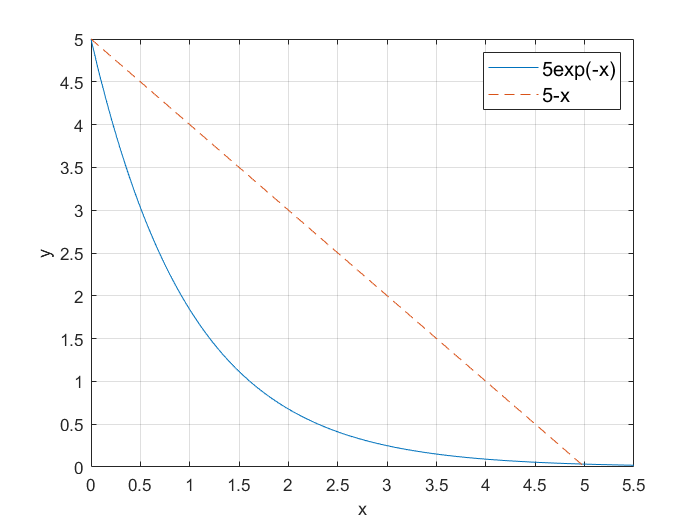
\includegraphics[scale=.5]{fig8-8.png}
\caption{第8.8题 图解法}
\end{figure}
\\可得$x=4.9651$,因此
\begin{equation}
\lambda_mT=\frac{hc}{4.9651k}
\end{equation}
$\lambda_m$随温度增加向短波方向移动。
\end{sol}

\begin{problem}{8.13}
银的导电电子数密度为$5.9\times10^{28}/m^3$,试求$0K$时电子气体的费米能级、费米速率和简并压。
\end{problem}
\begin{sol}
$0$K时电子气体的费米能量为
\begin{equation}
\mu_0=\frac{\hbar^2}{2m}\left(3\pi^2\frac{N}{V}\right)^{2/3}=\frac{(1.05\times10^{-34})^2}{2\times9.1\times10^{-31}}\left(3\pi^2\times5.9\times10^{28}\right)^{2/3}J=8.8\times10^{-19}J=5.5eV
\end{equation}
费米速率为
\begin{equation}
v_F=\frac{\hbar}{m}\left(3\pi^2\frac{N}{V}\right)^{1/3}=\frac{1.05\times10^{-34}}{9.1\times10^{-31}}\left(3\pi^2\times5.9\times10^{28}\right)^{1/3}m/s=1.4\times10^6m/s
\end{equation}
简并压为
\begin{equation}
p=\frac{2}{5}n\mu_0=\frac{2}{5}\times5.9\times10^{28}\times8.8\times10^{-19}Pa=2.1\times10^{10}Pa
\end{equation}
\end{sol}

\begin{problem}{8.17}
等温压缩系数$\kappa_T$和绝热压缩系数$\kappa_S$的定义分别为$\kappa_T=-\frac{1}{V}\left(\frac{\partial V}{\partial p}\right)_T$和$\kappa_S=-\frac{1}{V}\left(\frac{\partial V}{\partial p}\right)_S$[式(2.2.13)],试证明对于$0K$的理想费米气体,
\[
\kappa_T(0)=\kappa_S(0)=\frac{3}{2}\frac{1}{n\mu(0)}
\]
\end{problem}
\begin{sol}
$0$K下理想费米气体的简并压为
\begin{equation}
p(0)=\frac{2}{5}n\mu_0=\frac{\hbar^2}{5m}(3\pi^2)^{2/3}\left(\frac{N}{V}\right)^{5/3}
\end{equation}
等温压缩系数为
\begin{equation}
\kappa_T(0)=-\frac{1}{V}\left.\left(\frac{\partial V}{\partial p}\right)\right|_{T=0}=-\frac{1}{V}\frac{1}{\left(\left.\frac{\partial p}{\partial V}\right)\right|_{T=0}}=-\frac{1}{V}\frac{1}{\frac{\hbar^3}{5m}(3\pi^2)^{2/3}\left(\frac{N}{V}\right)^{5/3}\left(-\frac{5}{3}\frac{1}{V}\right)}=\frac{3}{2}\frac{1}{n\mu(0)}
\end{equation}
根据能斯特定理,$\lim_{T\Rightarrow0}S=0$,故
\begin{equation}
\left(\frac{\partial V}{\partial p}\right)_{T=0}=\left(\frac{\partial V}{\partial p}\right)_{S=0}
\end{equation}
从而绝热压缩系数为
\begin{equation}
\kappa_S(0)=-\frac{1}{V}\left(\frac{\partial V}{\partial p}\right)_S=-\frac{1}{V}\frac{1}{\left(\left.\frac{\partial p}{\partial V}\right)\right|_{T=0}}=\frac{3}{2}\frac{1}{n\mu(0)}
\end{equation}
\end{sol}

\begin{problem}{8.22}
由$N$个自旋极化的粒子组成的费米气体处在径向频率为$\omega_r$、轴向频率为$\lambda\omega_r$的磁光陷阱内,粒子的能量(哈密顿量)为
\[
\varepsilon=\frac{1}{2m}(p_x^2+p_y^2+p_z^2)+\frac{m}{2}\omega_r^2(x^2+y^2+\lambda^2z^2)
\]
试求$0K$时费米气体的化学势和粒子的平均能量。假设$N=10^5$,$\omega_r=3800s^{-1}$,$\lambda^2=8$,求出数值结果。
\end{problem}
\begin{sol}
取能量零点为$\hbar\varepsilon\left(1+\frac{\lambda}{2}\right)$,粒子的能量为
\begin{equation}
\varepsilon_{n_x,n_y,n_z}=\hbar\omega(n_x+n_y+\lambda n_z),\quad n_i=0,1,2,\cdots(i=x,y,z)
\end{equation}
化学势满足
\begin{equation}
N=\sum_{n_x,n_y,n_z}\frac{1}{e^{\beta[\hbar\omega(n_x+n_y+\lambda n_z)-\mu]}+1}
\end{equation}
当$N$足够大以至于$n_i$的足够多,上式可化为积分
\begin{equation}
N=\iiint\frac{dn_xdn_ydn_z}{e^{\beta[\hbar\omega_r(n_x+n_y+\lambda n_z)-\mu]}+1}
\end{equation}
令$\varepsilon_i=n_i\hbar\omega_r,(i=x,y)$,$\varepsilon_z=\lambda n_z\hbar\omega_z$,上式可化为
\begin{equation}
N=\frac{1}{\lambda(\hbar\omega_r)^3}\iiint\frac{d\varepsilon_xd\varepsilon_yd\varepsilon_z}{e^{\beta[(\varepsilon_x+\varepsilon_y+\varepsilon_z)-\mu]}+1}=\frac{1}{\lambda(\hbar\omega_r)^3}\iiint\frac{d\varepsilon d\varepsilon_xd\varepsilon_z}{e^{\beta(\varepsilon-\mu)}+1}
\end{equation}
其中$\varepsilon=\varepsilon_x+\varepsilon_y+\varepsilon_z$,对给定的$\varepsilon$,$\varepsilon_x+\varepsilon_y\leq\varepsilon$,$\int d\varepsilon_x\int d\varepsilon_y=\frac{1}{2}\varepsilon^2$,故上式可化为
\begin{equation}
N=\frac{1}{2\lambda(\hbar\omega_r)^3}\int_0^{+\infty}\frac{\varepsilon d\varepsilon}{2e^{\beta(\varepsilon-\mu)}+1}=\int_0^{+\infty}\frac{D(\varepsilon)d\varepsilon}{e^{\beta(\varepsilon-\mu)}+1}
\end{equation}
其中态密度$D(\varepsilon)d\varepsilon=\frac{1}{2\lambda(\hbar\omega_r)^3}\varepsilon^2d\varepsilon$。\\
$0$K时,所有粒子尽可能处于最低的能级,由于这是费米系统,故粒子将会从能量零点填充到费米能级$\mu(0)$,此时总粒子数为
\begin{equation}
N=\frac{1}{2\lambda(\hbar\omega_r)^3}\int_0^{\mu(0)}\varepsilon^2d\varepsilon=\frac{1}{2\lambda(\hbar\omega_r)^3}\frac{\mu^3(0)}{3}
\end{equation}
故此时费米气体的化学势为
\begin{equation}
\mu(0)=\hbar\omega_r(6\lambda N)^{1/3}
\end{equation}
粒子的平均能量为
\begin{equation}
\bar{\varepsilon}=\frac{1}{N}\int_0^{\mu(0)}D(\varepsilon)\varepsilon d\varepsilon=\frac{1}{2\lambda(\hbar\omega_r)^3}\frac{\mu^4(0)}{4}=\frac{3}{4}\mu(0)=\frac{3}{4}\hbar\omega_r(6\lambda N)^{1/3}
\end{equation}
代入题设数据得
\begin{gather}
\mu(0)=\hbar\omega_r(6\lambda N)^{1/3}=1.05\times10^{-34}\times3800\times(6\times2\sqrt{2}\times10^{5})^{1/3}J=4.8\times10^{-29}J\\
\bar{\varepsilon}=\frac{3}{4}\mu(0)=3.6\times10^{-29}J
\end{gather}
\end{sol}

\begin{problem}{8.23}
承上题,试求低温极限$T\ll T_F$和高温极限$T\gg T_F$下,磁光陷阱中理想费米气体的化学势、内能和热容。
\end{problem}
\begin{sol}
在低温极限$T\ll T_F$下,根据课本式(8.5.14),积分
\begin{equation}
I=\int_0^{+\infty}\frac{\eta(\varepsilon)}{e^{\frac{\varepsilon-\mu}{kT}}-1}d\varepsilon
\end{equation}
可展开为
\begin{equation}
I=\int_0^{\mu}\eta(\varepsilon)d\varepsilon+\frac{\pi^2}{6}(kT)^2\eta'(\mu)+\cdots
\end{equation}
故磁光陷阱中理想费米气体的总粒子数可写为
\begin{gather}
N\approx\frac{1}{6\lambda(\hbar\omega_r)^3}\mu^3\left[1+\pi^2\left(\frac{kT}{\mu}\right)^2\right]\\
\Longrightarrow\mu=(6\lambda N)^{1/3}(\hbar\omega_r)\left[1+\pi\left(\frac{kT}{\mu}\right)^2\right]\approx\mu(0)\left[1-\frac{\pi^2}{3}\left(\frac{kT}{\mu(0)}\right)^2\right]
\end{gather}
气体内能为
\begin{align}
\nonumber U=&\frac{1}{2\lambda(\hbar\omega_r)^3}\int_0^{+\infty}\frac{\varepsilon^3d\varepsilon}{e^{\frac{\varepsilon-\mu}{kT}}-1}\\
\nonumber\approx&\frac{1}{8\lambda(\hbar\omega_r)^3}\mu^4\left[1+2\pi^2\left(\frac{kT}{\mu}\right)^2\right]\\
\nonumber\approx&\frac{1}{8\lambda(\hbar\omega_r)^3}\mu^4(0)\left[1-\frac{\pi^2}{3}\left(\frac{kT}{\mu(0)}\right)^2\right]^4\cdot\left[1+2\pi^2\left(\frac{kT}{\mu(0)}\right)^2\right]\\
\approx&\frac{3}{4}N\mu(0)\left[1+\frac{2}{3}\pi^2\left(\frac{kT}{\mu(0)}\right)^2\right]
\end{align}
热容为
\begin{equation}
C=\frac{dU}{dT}=Nk\pi^2\frac{kT}{\mu(0)}
\end{equation}
在高温极限$T\gg T_F$下,有$e^{-\frac{\mu}{kT}}\approx e^{-\frac{T_F}{T}}\approx1$,系统配分函数为
\begin{align}
\nonumber Z_1=&\int_0^{+\infty}D(\varepsilon)e^{-\beta\varepsilon}d\varepsilon\\
\nonumber=&\frac{1}{2\lambda(\hbar\omega_r)^3}\int_0^{+\infty}e^{-\beta\varepsilon}\varepsilon^2d\varepsilon\\
=&\frac{1}{2\lambda(\hbar\omega_r)^3}\frac{2}{\beta^3}
\end{align}
内能为
\begin{equation}
U=-N\frac{\partial}{\partial\beta}\ln Z_1=3NkT
\end{equation}
热容为
\begin{equation}
C=\frac{dU}{dT}=3kN
\end{equation}
化学势为
\begin{equation}
\mu=-kT\ln\frac{Z_1}{N}=-kN\left[6\left(\frac{kT}{\mu(0)}\right)^3\right]
\end{equation}
\end{sol}
\end{document}